\documentclass[a4paper, 11pt]{article}

\usepackage[ mincrossrefs=999, style=numeric, backend=biber, url=false,
isbn=false, doi=false, ]{biblatex}

\addbibresource{references.bib}

\usepackage[margin=1in]{geometry} \usepackage[dvipsnames]{xcolor}
\usepackage[colorlinks]{hyperref} \usepackage{enumitem} \usepackage{amsfonts}

\usepackage{unicode-math}
\usepackage{stmaryrd}
\usepackage{amsfonts}
\usepackage{mathtools}
\usepackage{xspace}

\NewDocumentCommand{\codeword}{v}{%
\texttt{\textcolor{gray}{#1}}%
}

\NewDocumentCommand{\term}{v}{%
\texttt{\textcolor{blue}{#1}}%
}
\NewDocumentCommand{\keyword}{v}{%
\texttt{\textcolor{orange}{#1}}%
}

\usepackage{ stmaryrd }

% \usepackage{enumitem}
\setlist[itemize]{noitemsep, topsep=0pt}

\hypersetup{ citecolor=RoyalBlue }

\usepackage{fontspec}

\usepackage{titlesec}

\titlespacing\section{0pt}{4pt plus 2pt minus 2pt}{4pt plus 2pt minus 2pt}

\usepackage{graphicx} % for images
\usepackage{float} % for figure[H]

% \setmainfont{Linux Libertine} % \setsansfont{Linux Biolinum} % %
% \setmonofont[Scale=0.85]{PragmataPro Mono Liga}

\begin{document} \pagenumbering{gobble}

\begin{titlepage}

\vspace*{1cm}

\begin{center} \Large Paper Proposal : Steps towards syntactic and semantic
  safety guarantees for voice assistants in autonomous vehicles  \\ 

% gurantess robustness? 
% autonomous vehicles ?

\vspace{1.5cm}

\large Warrick Macmillan  \\
\large Marco, Matthew, Katya, ... \end{center}

\end{titlepage}

\section{Abstract} 

We introduce a grammar for a controlled natural language (CNL) to give
imperative commands to a voice assistant for a self-driving car to 
verify its behavior. We specifically seek to give the user of our
system assurances against substitution-based attacks, whereby synonyms can be
given the same meaning by imposing these conditions in how the parse trees (in
our case, abstract syntax trees (ASTs)) are formed. In addition, we map our
trees to a semantic form in an Agda implementation of linear temporal logic
(LTL), which has many applications in the specification and verification of the
behavior of robotics systems, particularly those with neural network components.
We see that simple, formal systems provide a useful model for verifying systems
with more a greater breadth of ``knowledge'' capable of more complex
interactions.

\section{Overview}

Perhaps the most pervasive question in the use and application of natural
language technologies, and one which exemplifies the boundary of the formal
methods versus statistical methods approaches in designing such technologies,
can be stated as follows : How does one optimize the system to provide for wide
coverage of the domain while ensuring that system is robust?

The statistical, data-oriented, and machine learning methods applied to NLP
which have made enormous gains over the past three decades often take a more
pragmatic approach : compromise robustness for wide coverage, as this means the
tools will be usable and usable by non-experts. The formal approaches in
computational linguistics, instead, are often more concerned with theoretical
explainability. Therefore, the developers of these systems seek predictable and
well-defined behavior for specific problem domains. Yet, these systems fail to
generalize without an explosion in complexity when presented with data outside
their domain. The fact that natural language both seems structured with respect
to rules, yet continuously breaks or introduces exceptions to these rules, makes
it exceedingly hard penetrate from either the data oriented or formalist
approach. This leads many researchers to ask the degree to which large amounts
of data can be augmented with theoretical knowledge about language to create
optimal and practical systems with respect to both breadth and depth of
coverage of language phenomena.

This problem acutely arises in when trying to design a voice assistant in the
domain of commanding controllable robotics, specifically, autonomous vehicles.
For the actions the vehicle takes, mostly the motion and path decisions, must be
formally specified or at the very least controlled via some computer system
subject to mathematical formalism. Assuming the user directing the vehicle isn't
aware of these formalisms, it is incredibly difficult to design a controller
capable of dealing with the breadth of language one may encounter in the wild.

The instructions an arbitrary user gives are not subject to the same
formalities. For they may leave out detail (``go into the other lane'' with
multiple lanes on either side), say something wrong (``go into the other lane''
on a single lane road), or give a command the controller should recognize as bad
(``drive into the car ahead''). Additionally, the controller may need to
recognize many ways many users may say ``the same thing'', that is the same with
respect to some semantic formalism. Ambiguity and noise are other considerations
to try to deal with (presumably through some dialogue system). Finally, there is
the possibility of adversarial attacks, which we'll detail more below.

We therefore analyze our big-picture question above in the following
sub-question : how can one map the manifold ways of presenting information to an
autonomous robot into a rigorous and formally verifiable subsystem which the
controlled can understand? Our proposed solution is to build a semantic parser
from natural language commands to Linear Temporal Logic, whereby we can filter
the many possible natural language commands into a ``canoncial subset'' which
are equivalent to (sets of) temporal logic formulas. The ``sets of'' clause
references the inevitable ambiguity of parses even from a big enough parser, even
if the size of the canoncial expressions is vastly smaller than the domain of
expressions mapping to them.

\begin{figure}[H]
\centering
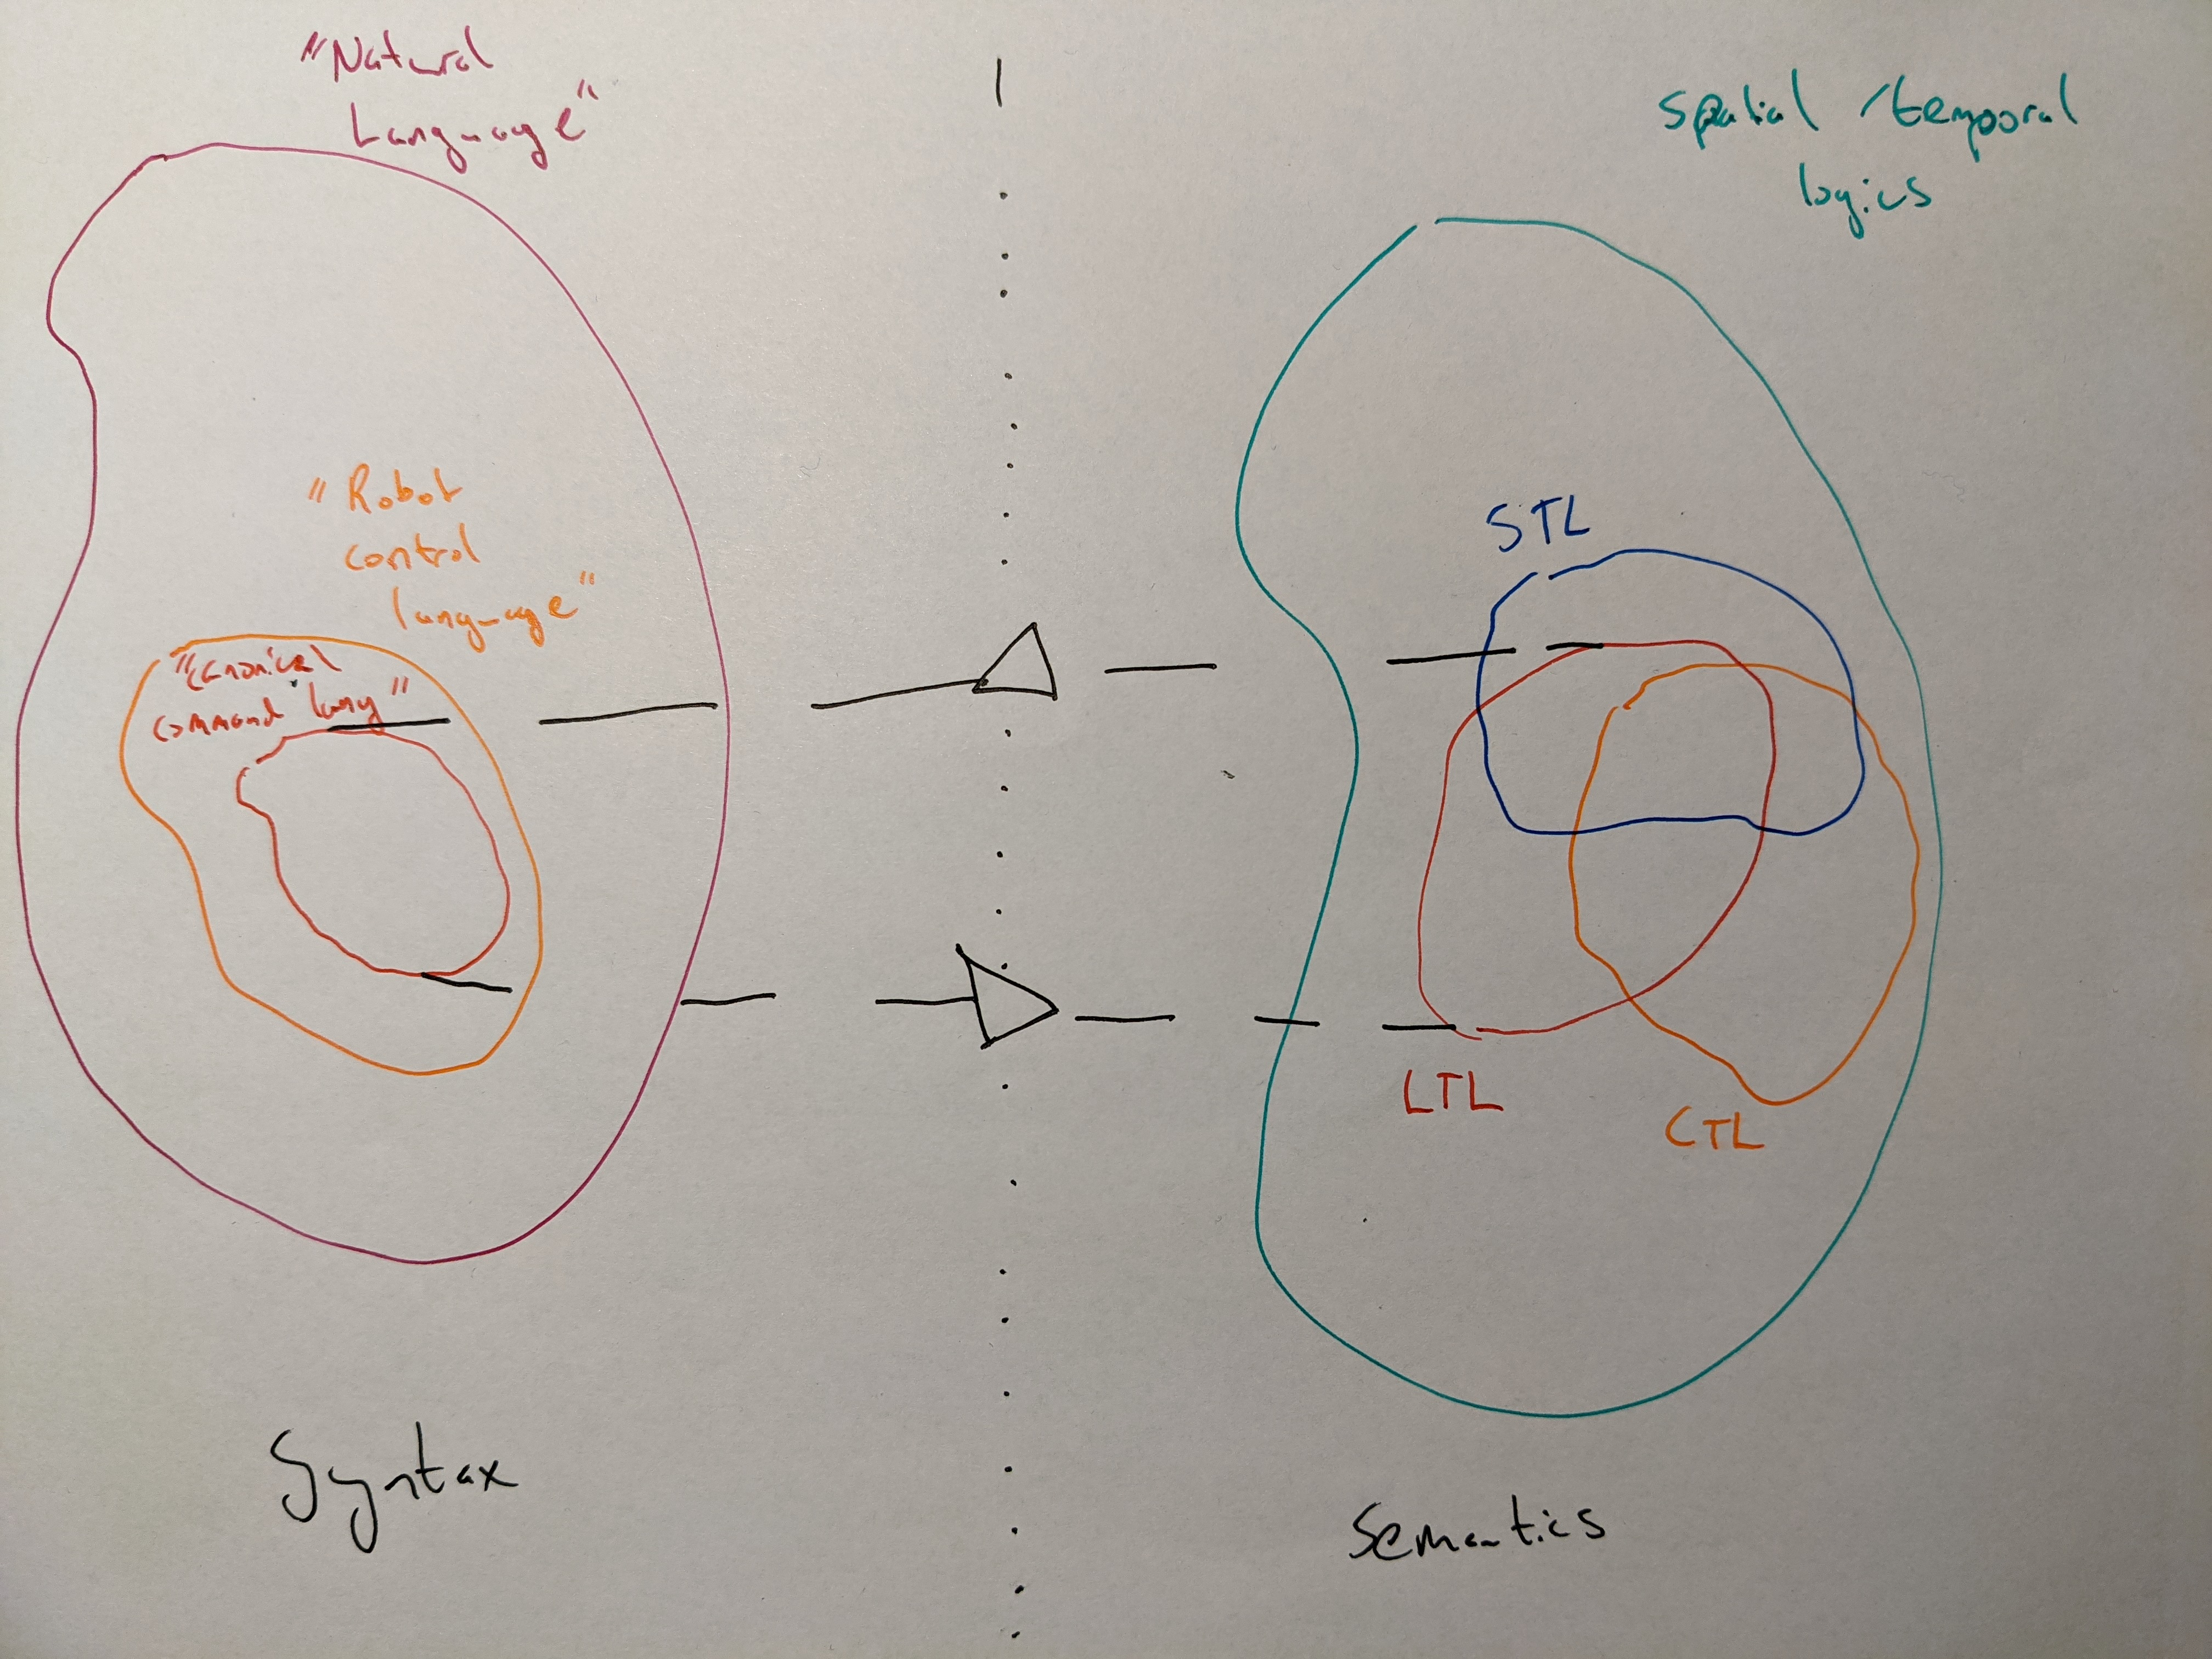
\includegraphics[width=150mm]{pics/one.jpg}
\caption{Language and Logical Spaces of Concern} \label{fig:M1}
\end{figure}

We begin in \autoref{fig:M1} with a high level overview of this semantic parsing
system, whereby the space of natural language syntax can be mapped to some
formal language semantic space (and possibly have some kind of inverse mapping).
We note that ``Natural Language'', while an idealized notion, can be thought of
the space of interpretable utterances. The relatively small subset of these
utterances which one might give to a robot, labeled ``Robot Control Language'',
is the ideal breadth our system would support, is still actually very large. We
therefore applying another filter, to the ``Canonical Command Language'' which
is inductively defined via some relatively thin set of grammar rules, which
simultaneously generate and parse expressions in some logic. Although we target
LTL because of its prominence in the literature and relatively straightforward
implementation and interpretation, it should be noted that their are other
temporal logics which may well be more expressive and better suited to the
actual problem of synthesizing controllers.

\begin{figure}
\centering
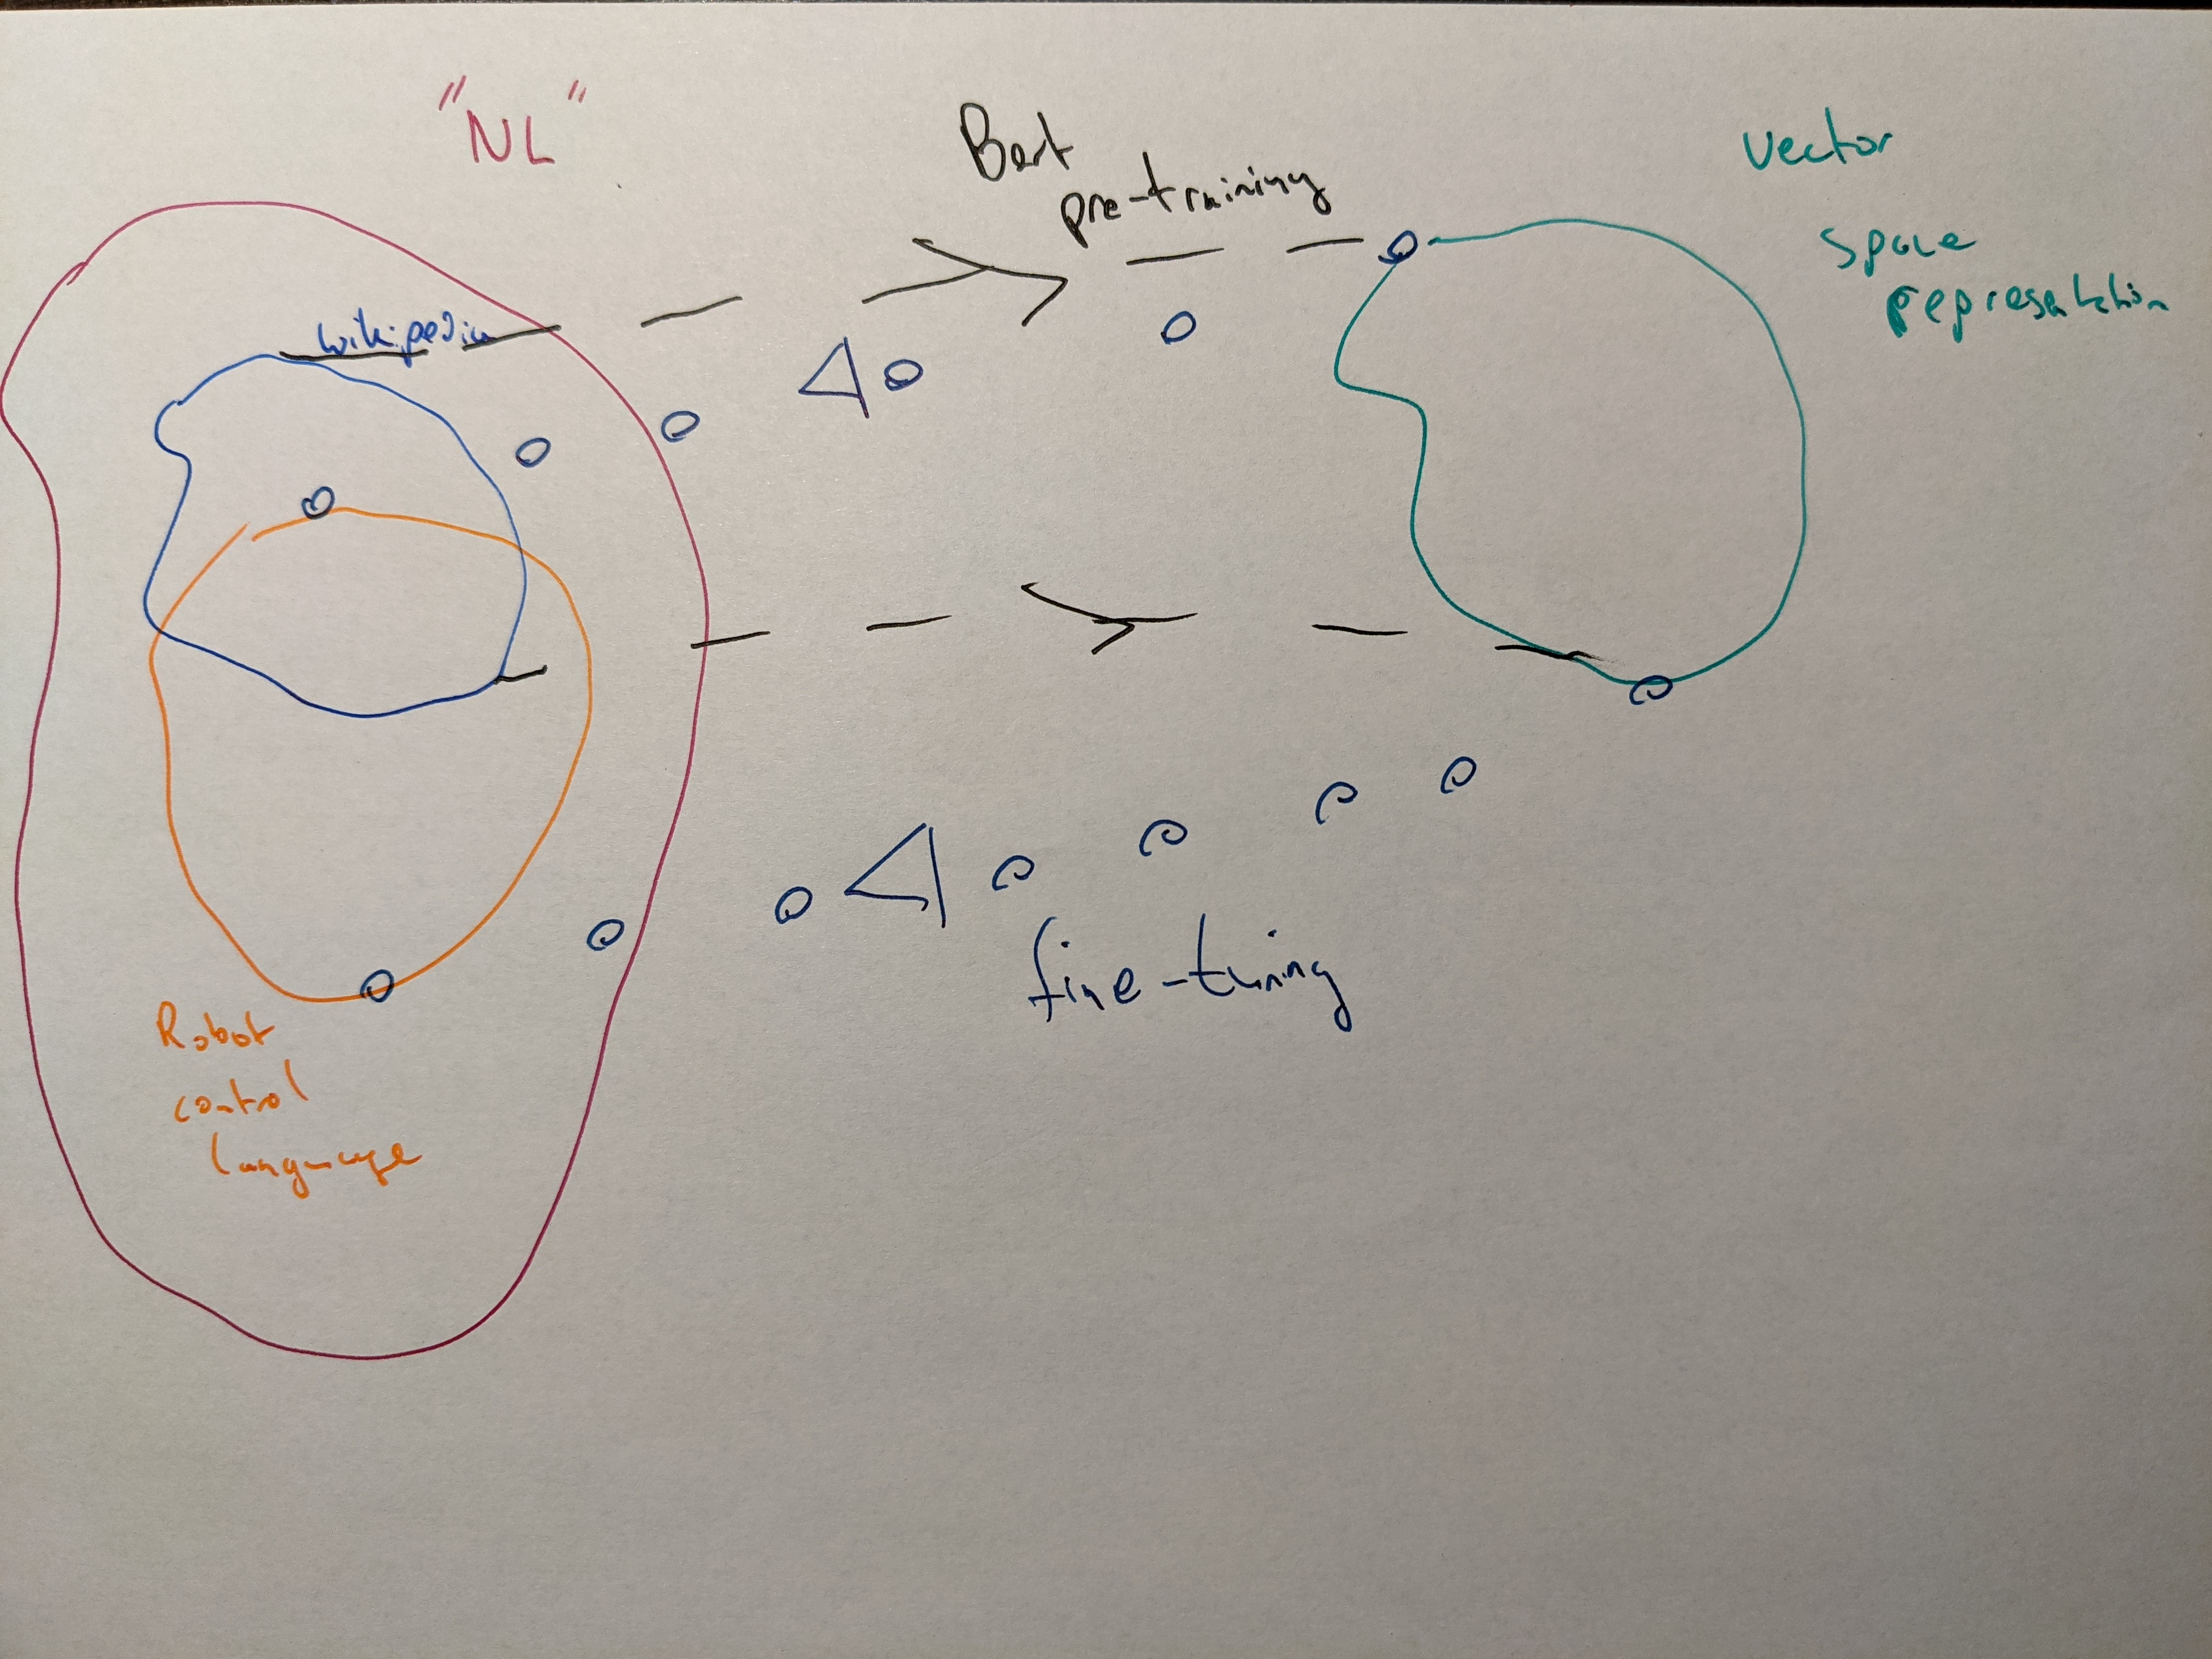
\includegraphics[width=150mm]{pics/two.jpg}
\caption{A simple caption}\label{fig:M2}
\end{figure}

Due to the recent influx of transformer based language models like Bert and
GPT3, we take for granted that the easiest way to target our ``Robot Control
Language'' will be through fine-tuning one of these models, as shown in
\autoref{fig:M2}. These transformers, trained on a separate corpus like
Wikepdia, can be mapped to some suitable set of robot commands, even though
these types of expressions will have a sparse presence in the corpus the model
was initially trained on (presumably Marco will know more about this than me).

In this context, we can then further refine the language to something less
natural, but more canonical. The whole proposed pipeline in \autoref{fig:M3},
indicates the methodology as interpreted from \cite{fewShotSem}, whereby the
semantic parser should ideally be able to taking any command from the Robot
Control Language and turn it into a set of temporal logic formulas, distributed
according to most likely interpretation.

Ideally, the downstream system should either be able to (i) ask for
clarification if two formulas are determined to be of some relative likelihood,
reject a formula that is not determined to be achievable (for whatever reason),
or synthesize a sequence of actions according to the possibly modified current
path. 

\begin{figure}
\centering
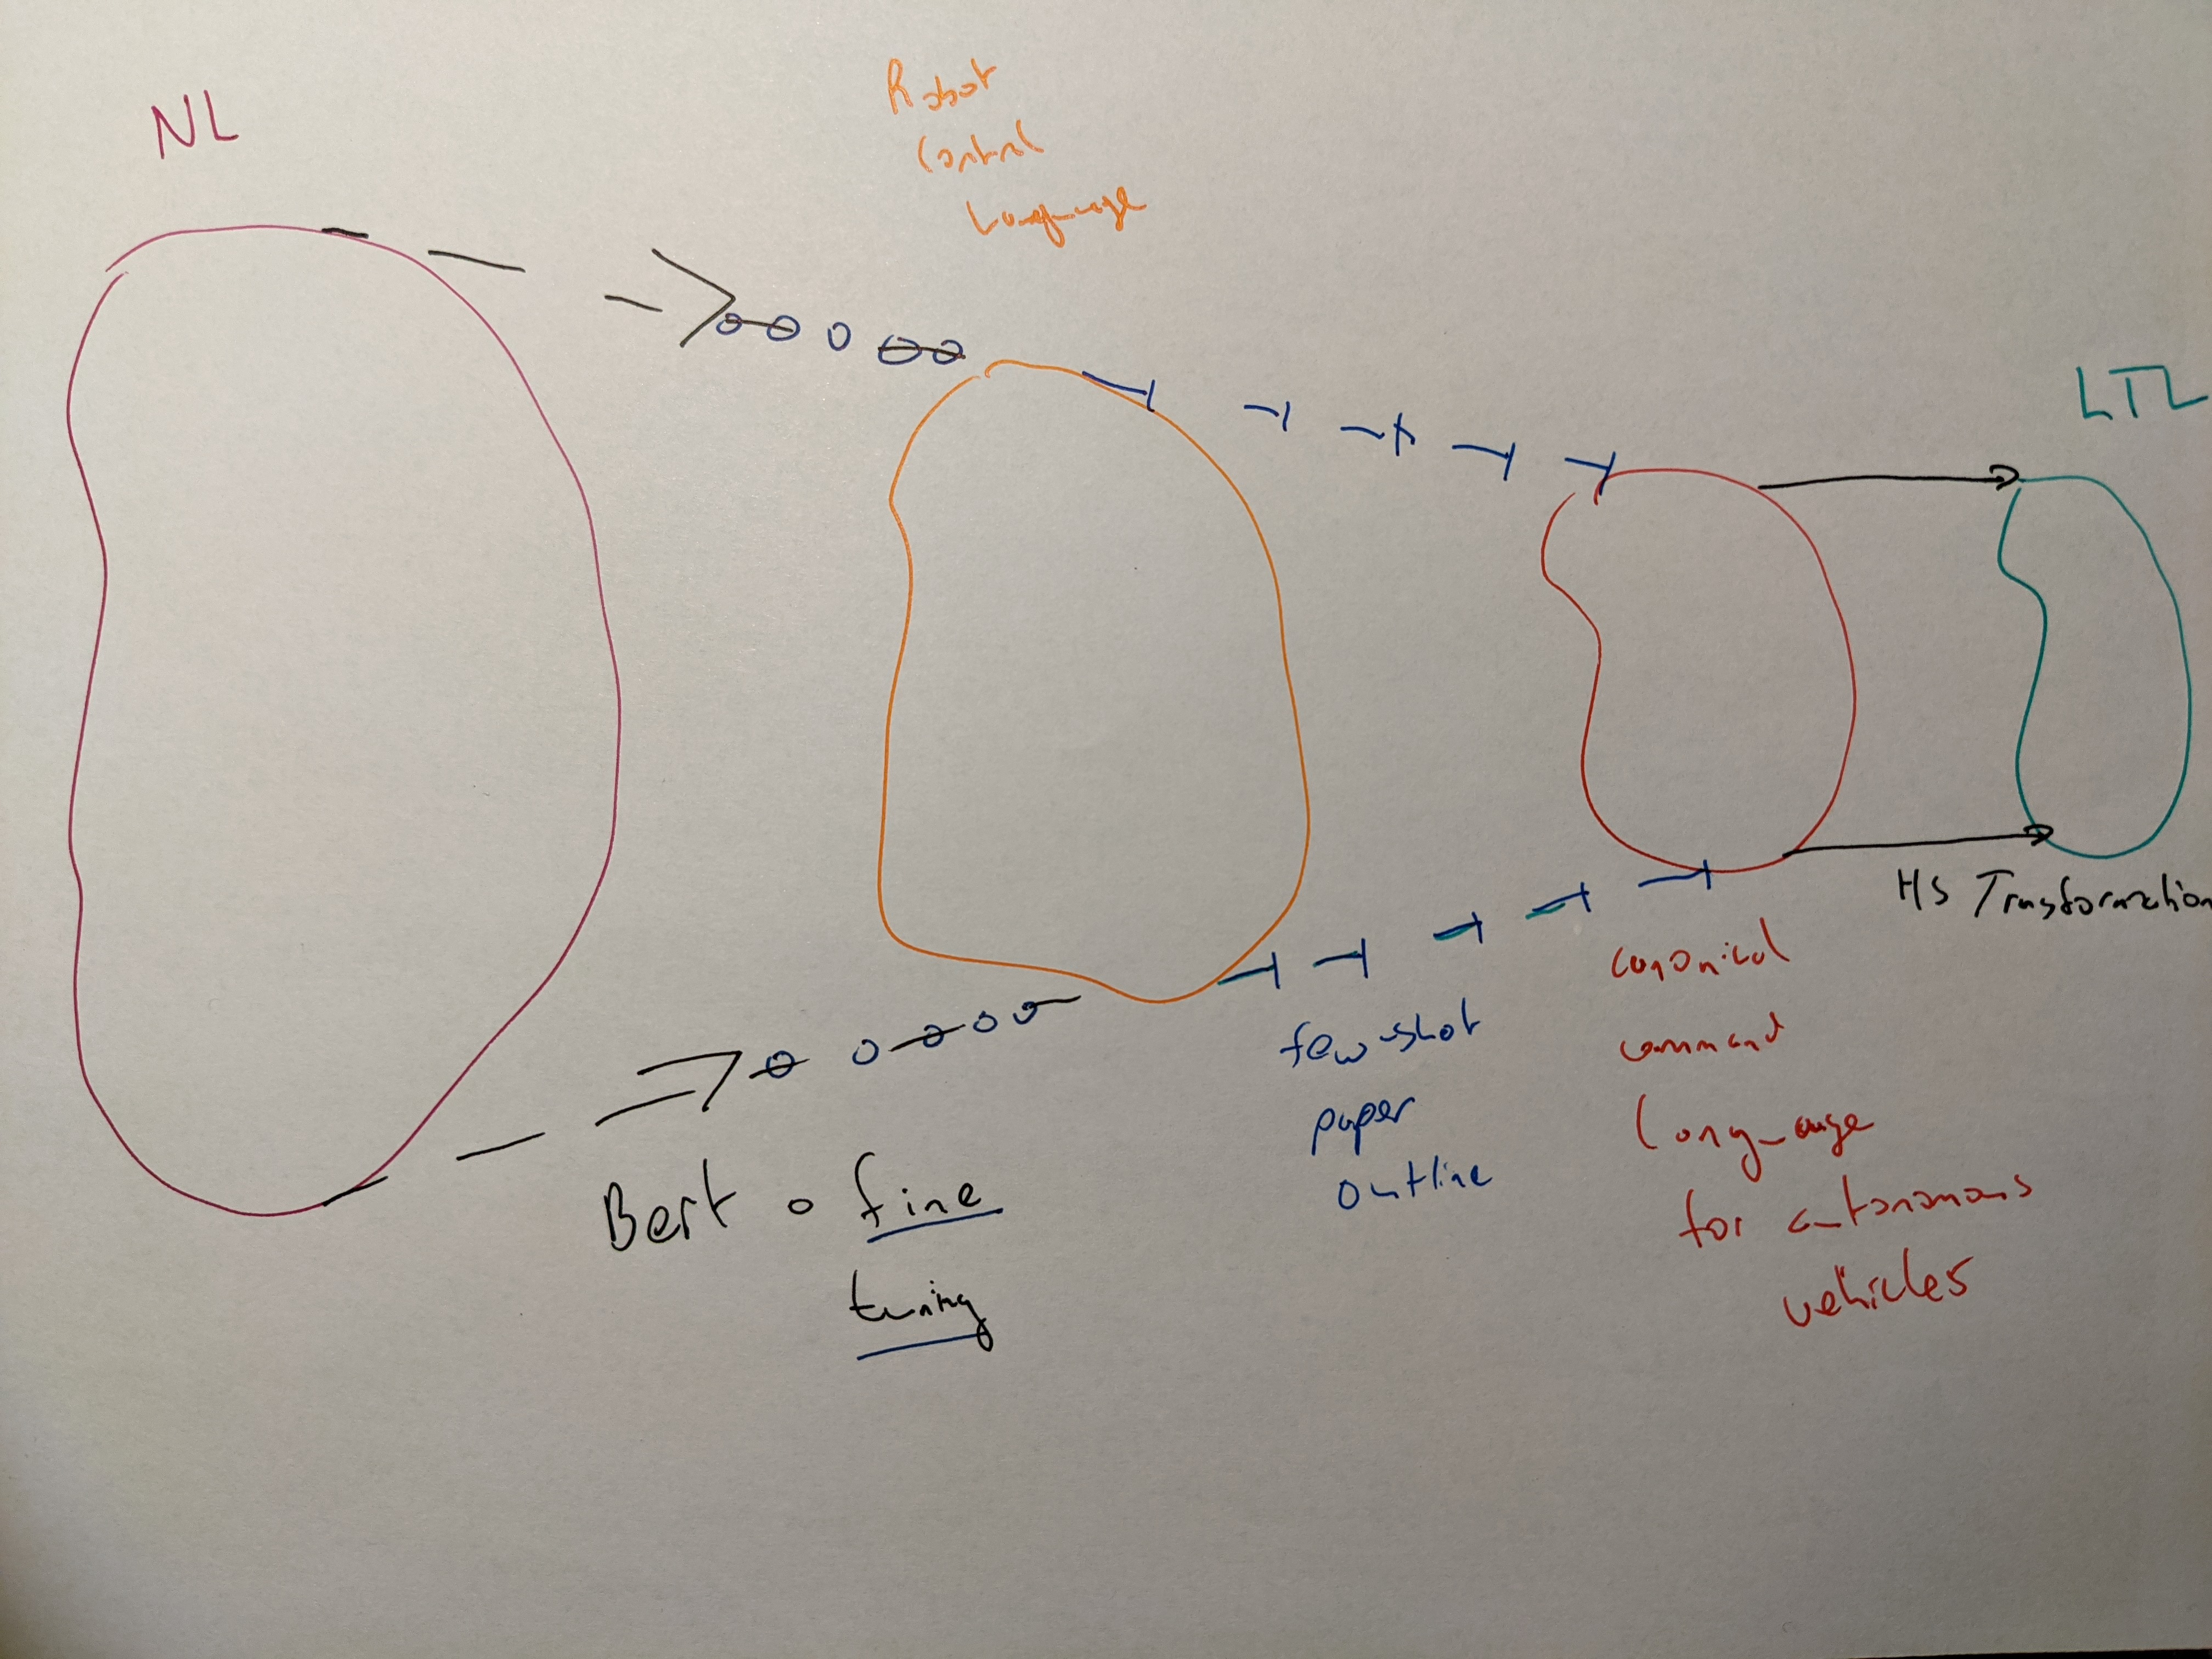
\includegraphics[width=150mm]{pics/three.jpg}
\caption{A simple caption}\label{fig:M3}
\end{figure}

In theory, we can embed clauses which in turn reflect all of natural language :
``Stop at the man who is watching the tv show on his phone about time traveler
who goes back to the 12th century Mongolia, whereby the man, not speaking
Mongolian ...'' This is clearly outside the boundary of what the robot control
language should support, and ideally would be accepted or rejected by the
computer prior to the commands completion depending if there was a man looking
at a phone. Our parser currently accepts strings in our primitive canonical
language such as

\begin{verbatim}
  p "drive to the store , turn right and stop at the dog"

  MultipleRoutes And (ConsPosCommand (SimpleCom (ModAction Drive (MkAdvPh To
  (WhichObject The Store)))) (BasePosCommand (SimpleCom (ModAction Turn
  (WherePhrase Right))) (SimpleCom (ModAction Stop (MkAdvPh At (WhichObject The
  Dog))))))
\end{verbatim}

However, we may envision our system being able to accept an expression in the
Robot Control Language like ``hit the petal till we come up to the store, hang a
right, and halt when you see a cute little puppy''. We could certainly adjust
our parser to accomodate this, but it would be one of many possible edge cases
unlikely to be uttered. To accomodate many more such edge cases would cause an
exponential blowup in the parser size (thereby slowing down parsing), but more
importantly, cause the programmer a headache when needing to map the parser to
the logical form. If we treat $F$ as the operating expressing the existence a
future state, $X$ as the next state, and $G$ meaning the universal future, our
desired LTL formula would most likely treat this as $F\ (store \land\ (X\
turn\_right\ \land\ (F\ (G\ dog))))$, although we propose that the actual
grounding of these to images or controllable actions to some downstream system.

LTL has been a popular logic for specifying controllable robot behaviors,
particularly with respect to verification of their behaviors. In
\cite{verifiedMotion}, Rizaldi et al. prove logical correctness of a motion
planner with respect to LTL formulas over maneuver automata formulas in the
Isabelle/HOL theorem prover, a non-dependent cousin of Agda. We are choosing to
deeply embed LTL in Agda for a few reasons, although the syntax of the embedding
could easily be translated to any other dependently typed theorem prover, and
with a little more effort probably any functional programming language. The
composition of a ``weakly verified'' natural language front-end with a formally
verified back-end such as in Rizaldi's work would pave the way for a fully
verified, utterance to vehicle path streamline for the autonomous vehicles.

The big question to address is what kind of verification conditions the natural
language component should be subjected to, and what kind of attacks would be
most important to preemptively anticipate. Substitution based attacks
\cite{substAttacks}, for instance, have been consistently emphasized throughout
our discussions so far. The question is, \emph{where} in the pipeline it would
be best to filter out the vulnerabilities, as well as \emph{how}.

One possibility would be to define words modulo equivalent meanings using
Wordnet \cite{wordnet} in the syntactic phase, either via training
\cite{ren-etal-2019-generating} (presumably during the fine-tuning to the Robot
Command Language or our ``canonicalization'' from that). It has been suggested
that Bert is already relatively robust against such attacks
\cite{hauser2021bert}, but we nonetheless feel that even higher sensitivities of
robustness may be better done at other phases in the pipeline.

Alternatively, one could just map these equivalent Wordnet forms to equivalent
parse trees using the Portable Grammar Format (PGF) Haskell library, which
essentially deeply embeds a GF grammar into a Generalized Algebraic Datatype
(GADT).

For instance, if we abstract over all abstract syntax trees for our grammar
using this library, we can define the following Haskell functions to equate a
``female human'' with a ``woman''. 

\begin{verbatim}
treeMapfemalePersonIsWoman :: forall a. Tree a -> Tree a
treeMapfemalePersonIsWoman (GModObj GFemale GPerson) = GWoman
treeMapfemalePersonIsWoman GWoman                    = (GModObj GFemale GPerson)
treeMapfemalePersonIsWoman gp = composOp treeMapfemalePersonIsWoman gp
\end{verbatim}

There has been work integrating multiple language Wordnets with GF
\cite{virk2014developing}, so it would presumably be easy to integrate with our
system, depending on how large we want the grammar to get.

We could also try to classify similar trees at the semantic level, i.e. cluster
similar LTL formulas. Katya has suggested we could do something in line with her
and Heras' work on Machine Learning for Proof General (ML4PG) \cite{ml4pg}. 

As it is unclear what the best direction for this is, and how the attacker model
in the context of an autonomous vehicle might work, all these decisions need to
be made in the context of discussions within the group.

\section{Introduction}

While the evaluation of machine learning systems provides assurances using
different scores and metrics on different tasks assures one they may on average
perform better than humans at certain tasks, the advent of adversarial attacks
\cite{szegedy} with the intention of deceiving such a system by a hostile actor
leads the system designer to desire, and possible require additional
verification about the system's behavior. In the context of natural language
processing (NLP), where data sources rely on strings of text, these attacks can
focus an array of features from spellings of individual words to rearranging
entire sentences \cite{}. So-called synonym attacks, which adversarially target
the system at the lexical level, can cause traditional NLP models to [...]
\cite{}.

In the context of designing a voice assistant for an autonomous vehicle, whereby
one can give commands like ``turn right after the woman with the big dog",
we desire that the intensional belief a user has about her utterance is
consistent with the extensional behavior of the vehicle. This can be done
through an intermediary mapping to a formal semantic representation. Ensuring
that the syntactic content of a voice director's (well-formed) utterance maps predictably to
the logical form is important from the verificationist perspective : one wants
to maximize the ``syntactic completeness" of the system \cite{macmillan2021}.

Aside from the user experience being compromised by a system which has been
adversarially afflicted, there is also a possibility of physical danger for the
passenger and other people in the vicinity. As voice directed robots have many
possible points of failure, we focus on two types of verification for our
system. Rather than focus on breadth of language coverage, which ML language
models excel at of due to their reliance on statistical modeling and tons
of data, our system is narrowly focused as a proof-of-concept, from which it
could either be extended by hand, or different components modified using
other techniques and tools.

\section{Current Landscape} 

\subsection{Voice assistants for autonomous vehicles}

The public company Cerence \cite{} is already designing voice assistants for autonomous
vehicles, for which it has a large software stack between the voice processing
to actual control of current automative components. In addition to its 
technologies, many of which aren't accessible to external researchers due to
intellectual property restrictions, Cerence has contracts with large automakers
[..]. It is therefore natural to inquire, what a small team with varied
backgrounds and not nearly the same expertise nor experience within the
technological team at Cerence can provide.

First, we believe that the focus on verification, insofar as we envision it, is
unlikely to be of current concern at Cerence due to the fact that their products
are still being developed, and the primary goal of producing a working product
is likely to precedence over preventing non-existent hostile actors.

Additionally, it is going to have to be determined by 
[verification of self-driving cars generally : software, hardware, behavior in
a real environment, etc]


\subsection{Natural Language and Robots, generally}

\subsection{Semantic Representations of NL for verification}

Modal logics, specifically those dealing with time like LTL, CTL, STL, ..., have
been used extensively in the specification and verification of properties of
robotics systems, including autonomous vehicles [cite]

With verification being a core motivation of our work, we take for granted that
these different logics have many manifestations in different systems. However,
we hope that by choosing a domain with a lot of attention, that our system can
be generalized in many possible directions :

\begin{itemize}
\item other logics
\item other parsing formalisms (perhaps dependency for wide-coverage)
\item other syntax -> semantic formalisms
\item other robotics domains
\end{itemize}


\subsection{Foundation Models}

\section{Work} 

\subsection{GF Grammar}

\section{TODO} 

\subsection{Grammar modulo wordnet}

\subsection{LTL in Agda}

Along with colleagues from Singapore Management University, we have begun an
Agda implementation \cite{wltl} of LTL which will serve as the semantic space
for our parsed utterances. Our method, uses a deep embedding, as opposed to the
shallow embedding in \cite{coqLTL}, although the temporal encoding of paths as
streams was directly adapted from this paper.

This implementation will hopefully allow us to prove decidability of LTL in a
relatively straightforward manner. Other than the assurance that our
implementation is correct, we hope this will allow us to feed the formula into
some SAT or SMT solver so-as to actually allow verification of the behavior of a
vehicle with respect to an utterance.

[TODO : Help from Matthew?]

\subsection{AST -> Agda}

\subsection{ML training/verification stuff}
Help from Marco, Nathalia if interested?


\section{Publications Description}

Realizing that the structure of the paper is ameanable to large changes, I'm
posting a summary of relevant publications here.

\subsection{Statistical (pre-trained) Language Models}
The first set of publ

\begin{itemize}

\item In \cite{fewShotSem} [under review], the authors show how, using a \emph{synchronous
context-free grammar} (SCFG) to define a minified CNL with a parallel and dually
parsible semantic form, that one can use a large pre-trained language model as a front-end
to filter a much wider syntax into the CNL. I postulate GF's expressivity is
more expressive than the SCFG, at least based off a tertiary reading in the
index, and therefore if we carved out a subset of commands to cohere with our
LTL (and maybe some other temporal or even spatial-temporal logics in the
future), our model would be amenable to a similar ``out-of-the box" semantic
parser that could actually be used for verification. This paper borrows the idea
of ``semantic parsing as paraphrasing'' from  \cite{berant-liang-2014-semantic}

\item In \cite{dontParse}, the authors advocate for getting rid of parsers
  alltogether, although this naively takes for granted large public data-sets,
  none of which exist for an autonomous vehicle and temporal logic formalism
\item  \cite{hauser2021bert} [under review] claims that Bert is robust, analyzing claims of four
  papers, including the one which uses a wordnet attack

\end{itemize}

\subsection{NL to TL}

Here we show mainly relevant research for NL to LTL.

The applications of LTL in machine learning are vast, and the scope of our
specific application is still unclear, but nevertheless, we give a literature
review of methods and applications relevant for our work.

\begin{itemize}



\item This paper \cite{5152776} from 2009 uses a categorial grammar approach, but more or less
  can serve as an idea template for us, also nice pictures with grammar rules
  and formulas
\item Also, a highly relevant template combines Natural Language, LTL, with the
  idea of having a verifiable pipeline \cite{provCorrectNatControl} 

\begin{quote}
The production of an on-
tology of common actions and the type of formulas that
they produce—for example, safety conditions, adding goals,
constraining the initial state—in their negated and positive
forms would be a step toward a more general solution to
the problem of mapping natural language to LTL. Previous
work has relied heavily on grammar formalisms to ease...
\cite{provCorrectNatControl} 
\end{quote}

\item LTL formulas can be transformed into automata which can then be used as reward functions for reinforcement learners, as in \cite{ltlRein}

\item  The following is one of the more relevant quotes from a paper reviewing
  the whole space of English to LTL translations
  \begin{quote}
Overall, the typical approach followed by these studies can be summarized as follows:
given an input English utterance, preprocess it to extract syntactical information, which may
include part of speech tagging, dependency parsing, semantic role labelling, and so on. Then,
enrich the input with these pieces of information. Finally, run an attribute grammar-based
parser, or rely on some hand-made rules, to derive a translation into a target logical format.
A notable exception is the work of [89], where a fully-supervised learning setting is considered.
\cite{brunello_et_al}
\end{quote}
\item Translating between English and STL can be done via a large language model 
\cite{he2021english} [under review], but the domain specificity of the problems
are still significant enough to suggest that it will be years before an
automated semantic parser is available, if it is even possible. 
\item Could ask Lapata in Edinburgh, whose work \cite{dong-lapata-2016-language}
  is relevant and well-cited (although they use an encoder-decoder method)
\item
\item
\item

\end{itemize}

\subsection{Tellex}

Stephanie Tellex has written extensively about natural language inputs and
interfaces with robots. Although she has not specifically written about
autonomous vehicles, the domains have enough intersection to warrant careful
consideration of much of her work, especially the recent stuff.

\begin{itemize}

\item Grounding with an intermediate symbolic state, no LTL, but possibly
  relevant for paper generally. She also cites \cite{walkTalk}, a seminal paper in this area
\begin{quote}
Instruction following is a supervised learning problem
where the agent must predict a trajectory that would satisfy an
input natural language command. \cite{tellexInstr}
\end{quote}
\item The review paper \cite{MARGE2022101255} making recommendations has a
  section on robustness, but this is mostly for the sake of allowing sharing of
  interfaces and efficacy, no mention of verification (which is what we're
  primarily after)
\item They design a NL -> LTL for drones that are grounded to actual landmarks \cite{9197068}
\item The group builds a trained pipeline that uses an object oriented
  template-instance methodology to generalize to different ontological
  categories in  \cite{hsiung2021generalizing} [under review]

\item In \cite{patellearning} build learn a semantic parser from NL to LTL (so
that the language is grounded) where they collect executions of the LTL formulas
in different environments using a weakly-supervised training method with
reinforcement learning Part if the paper has to do with the execution of the
command being dependent on the path taken by the robot executing the command,
not just meeting the goal requirements, thereby giving a complexity bonus in
comparison to previous work. She also evaluates the model on the \cite{walkTalk}
data set
\end{itemize}

\subsection{Robot Motion Planning}

Without getting to into the weeds, for the actual planning and control of the
robot should, at least hypothetically, be at least somewhat 

\begin{quote}
  Robot motion planning and control is the problem of automatic construction of
robot control strategies from task specifications given in high-level, human-like language. The challenge
in this area is the development of computationally efficient frameworks allowing for systematic, provably
correct, control design accommodating both the robot constraints and the complexity of the environment,
while at the same time allowing for expressive task specifications.
\cite{4141034}
\end{quote}

\begin{itemize}
\item For instance, in \cite{plaku2016motion} the authors indicate how to actually
ground basic propositions from the language to paths in a space, while our
model, outputting formulas un-grounded base predicates, is merely concerned with
the logical structure.

\item 
\item In \cite{7759412}, the authors borrow the English to LTL pipeline from the
  aforementioned \cite{provCorrectNatControl}, and synthesize grounded controllers 
\end{itemize}

There is a group at MIT (Kuo, Katz, Barbu, ..) doing seemingly similar things to
Tellex's group.

\begin{itemize}
\item In \cite{kuo2020deep}, the authors do the most general end-to-end task
  without intermediary states,
  namely, map natural language commands to navigation and manipulation tasks.
  While this ``cutting out the middle man'' mentality may be an idealistic
  long-term vision, it makes the system much too much of a black box - for the
  fine-tuned verification conditions we desire to express and impose via the
  intermediate symbolic representations, the intermediate states, we imagine
  give us a more explainable, predictable, and regulatable system
\item More similar to Tellex et al's approach \cite{patellearning},
  \cite{ltlSemParse} seek to train a model via images in a simulated world.
  Their work also uses a SCFG (to generate semantically inadequate sentences
  with corresponding LTL formulas) from which they can direct machines to
  follow the instructions, and then have users describe the instructions in more
  natural form. 
\item One of the 
\end{itemize}



\printbibliography


\end{document}

